\documentclass[11pt]{article}
\pdfpagewidth 210mm
\pdfpageheight 297mm
\setlength\topmargin{0in}
\setlength\headheight{0in}
\setlength\headsep{0in}
\setlength\textheight{9.0in}
\setlength\textwidth{6.0in}
\setlength\oddsidemargin{0in}
\setlength\evensidemargin{0in}
\usepackage{cite}
\usepackage{verbatim}
\usepackage{amsthm,amssymb,amsmath}
\usepackage[pdftex]{graphicx}
\usepackage{float}
\floatstyle{boxed} 
\restylefloat{figure}
\begin{document}

\title{Computational Linguistics Assignment}
\author{Candidate 680817}
\maketitle

\section*{Question 1 (Incremental Parsing with the Perceptron Algorithm)}
\subsection*{Main features}
(Collins and Roark 2004)\cite{Collins2004} describes a statistical approach to parsing
natural language sentences based on machine learning techniques (the perceptron
learning algorithm). 

As with any such approach, the method requires a preliminary stage in which the
system is trained on a set of examples. 

\begin{figure}[h]
   \caption{Excerpt from (Collins and Roark 2004) describing a linear model for NLP}
   \begin{itemize}
   \item{Training examples $(x_i, y_i)$ for $i = 1 \dots n$}
   \item{A function \textbf{GEN} which enumerates a set of candidates $\textbf{GEN}(x)$ for an input $x$.}
   \item{
   A representation $\Phi$ mapping each $(x, y) \in \mathcal{X} \times
   \mathcal{Y}$ to a feature vector $\Phi(x, y) \in \mathbb{R}^d$ (where
   $\mathcal{X}$ and $\mathcal{Y}$ are the sets of inputs and outputs
   respectively).
   }
   \item{A parameter vector $\bar{\alpha} \in \mathbb{R}^d$}
   \end{itemize}
\end{figure}

In the linear model for NLP used, the question of training equates to finding
the `best' parameter vector $\bar{\alpha}$, where `best' can be taken to mean
the parameters which, when used in the incremental parsing algorithm as applied
to the input sentences of the training data, will most closely produce the
corresponding expected output parses.
\footnote{
In fact, Theorem 1 of \cite{Collins2004} states only that the training method does
this when the example data is separable. However, as they note, stronger
guarantees can be obtained via \cite{Freund1999} and \cite{Collins2002}.
}

Crucially, the examples are transformed by a \emph{representation} function
$\Phi$, which aims to capture the significant features of a parse tree.

See below for a more detailed description of the training process.

\subsection*{Data Requirements}

\subsubsection*{External input}
The training data will consist of sentences paired with their corresponding
correct parse trees.  The system will clearly also need to be given some
sentences to parse.

The final input data required is the grammar used to generate the list of valid parse candidates (\textbf{GEN}) - this could be induced from the training data or a larger corpus.

\subsubsection*{Internal data structures}

The goal of the training stage is to produce a parameter vector containing
perceptron weights. Since the only operation required on this vector is a
scalar product, it can be simply stored as an array.

Depending on the implementation, the set of features used for classification
might be considered to be data - however, it is probably safe to assume that
this is hard-coded.

\subsection*{Training}

The representation function maps from a sentence paired with a corresponding
candidate parse tree into a real vector space with dimension equal to the
number of discrete features under consideration.

The parameter vector $\bar{\alpha}$ encodes the weights of a single-layer
perceptron which is to be trained to separate correct parses for a sentence (as
seen by the representation function) from incorrect ones.  This means that
$\bar{\alpha}$ will come to encode the relative significance (positive or
negative) of each feature in performing this classification.

The feature set primarily consists of labels which refer to relative positions
in the parse tree. There are also some special features such as a flag
indicating the presence or otherwise of a question mark, and labels for the
lexical head of the constituent and similar significant nodes.

To train an example $(x, y)$, firstly $y$ is transformed to remove
left-recursion (see below). Then the system iterates through the words of $x$;
at each word, the relevant features are checked for. A present feature implies
that the representation function will have the value $1$ in the dimension
corresponding to that feature; absent features have $0$. This is how the output
of the representation function is calculated - this is then used in the
averaged perceptron algorithm as described in the paper.

One great advantage of perceptron training in this situation is that it is
generally \emph{faster} than a lot of other machine learning techniques - such
as maximum entropy classifiers or support vector machines - and this is
important when dealing with the large corpora necessary for training an
effective natural language parser for any real-world purposes.

(Collins and Roark 2004)\cite{Collins2004} also use two refinements to this
training system, for greater efficiency: repeated use of hypotheses, and `early
update'. The former involves keeping a cache of examples, and reiterating over
them to prevent errors from being introduced. The latter concerns the point at
which the parameters are updated. In the case where the parameters being used
in the training process are bad to the extent that using them as part of the
beam-search heuristic results in the desired parse not being found at all, the
parameters are updated immediately rather than at the end of the sentence. This
takes advantage of the greater information available at that time, and produces
a significant improvement in accuracy.


\subsubsection*{Averaged Perceptron Improvement}

The simplest training method involves repeatedly running the basic perceptron
algorithm on the example data either a fixed number of times or until a set of
weights is found which produces no errors on the example set. An alternative is
to use an average of the parameter values, sampled after each example has been
processed. Intuitively, this is a good idea since it reduces the degree to
which the produced parameters depend on the ordering of the example data (which
ought not to be significant).

As described in (Collins 2004)\cite{Collins2004}, the averaged perceptron
approximates Freund and Schapire's\cite{Freund1999} \emph{voted perceptron}
method.  The essence of the voted perceptron method is that the perceptron
algorithm is applied as if to every training example individually, producing a
whole array of corresponding parameter vectors. When later using the perceptron
to find the best parse of a sentence, each of these parameter sets are tried
separately, and the final parse chosen is the one which occurs most frequently
in the results of this.

\subsubsection*{Parsing}
Parsing can be seen as the problem of searching the space of possible parse
trees for a sentence for the one which scores best according to the model
trained from the example data. This space can be very large, but the perceptron
approach allows for a heuristic search strategy. The parser proceeds
incrementally, from left to right through the sentence. After each word, the
score for each candidate parse under the perceptron model is calculated, and
the candidates can then be filtered based on these scores. 

In training we can think of the perceptron as a linear classifier, but for
parsing we are interested in more than a simple boolean decision about whether
a parse is good or not; we wish to find the \emph{best} parse for a sentence
$x$. This is in fact the parse $z$ for which the vector $\Phi(x, z)$ is closest
to being perpendicular to the hyperplane which forms the perceptron's decision
boundary. Hence we seek $\operatorname{arg max}_{z \in \textbf{GEN}(x)} \Phi(x, z) \cdot \bar{\alpha}$.

`Decoding' is the process of trying to find the parse $z$ of a sentence $x$ which maximises the value of $\Phi(x,z) \cdot \bar{\alpha}$. This where the search procedure is required.

The filtering process after each word has been processed means that the overall
strategy amounts to a beam search: low-scoring partial hypotheses will be
dropped from consideration to ensure that space and time costs remain
manageable. When dealing with grammars sufficiently large to be useful for
general parsing, this is essential in order to make the problem tractable.

The filter used is essentially a threshold whose level increases with the cube
of the rank of the hypothesis. This means that lower ranked hypothesis are much
more likely to be dropped, and reflects a general `level of confidence' in the
heuristic. If the top ranked hypotheses have similar scores, they will most
likely all be kept - if one hypothesis outshines the rest, then perhaps only
that one will be used.

The other main component of the parser is the `advance' function, ADV. This
determines how the nodes of the hypothesis space are expanded - it can be
considered an efficient way of computing adjacency in this graph. Formally, ADV
should be equivalent to a function returning the elements of $\textbf{GEN}$
which differ from its argument only in the position of the word being added.
Computing this by brute force would be intractable due to the size of
$\textbf{GEN}$. Instead, we use the fact that any word being added to the right
of the sentence must be added to the parse tree by attachment to one of its
`left-child chains'. So we need only check all of the possible attachment sites
for each of these such chains. The left-child chains can be enumerated
exhaustively by a left-right breadth first search (or similar) of the
transformed grammar.

This gives us our new set of expanded partial hypotheses, whose scores are
calculated according to the perceptron. FILTER is applied, and the results are
expanded again, and so on, for the whole of the sentence.  The final stage is
to de-transform and return the parse tree of the top-ranked hypothesis for the
full sentence.

\subsubsection*{Grammar Transformations}

Although using beam search makes the problem more tractable, there may still be
very many possible parses to consider at each iteration of the search, depending
on the grammar used in the generation of candidates. The technique of
\emph{grammar transformations} is employed to ameliorate these difficulties.
The general aim is to restrict the left-child chains of the grammar in both
number and length.

The transform used first is a left-corner transformation, which removes
left-recursion from the grammar. This is essential because otherwise the number
of left-child chains will be infinite, and the process of enumerating them will
not even terminate\cite{Roark2001}. The details of an efficient method for this
are given by (Moore 2000)\cite{Moore2000}, although for our purposes we only
wish to transform rules which are actually left-recursive productions.

The second transformation is a flattening which unambiguously removes parent nodes, reducing the amount of space required.




\section*{Question 2 (Synchronous Context-free Grammars)}

In order to maintain proper subject-verb agreement in translation output, we
divide verbs according whether they will be followed by a definite article
(the/les), partative article (of-the/du), or that/que. This increases the
complexity of the grammar, but should prevent `ungrammatical' sentences from
being generated.
Similarly, nouns have separate rules for their different genders and for the plural.

\small
\begin{verbatim}
(Root sentence rule)
S -> <PROPER-NOUN[1] VERB-PHRASE[2], PROPER-NOUN[1] VERB-PHRASE[2]>

(Proper nouns)
PROPER-NOUN -> <John, John>
PROPER-NOUN -> <Pierre, Pierre>
PROPER-NOUN -> <Maria, Maria>
PROPER-NOUN -> <James, James>

(Three types of verb phrase; one for each verb type)
VERB-PHRASE -> <VERB-PRESENT-D[1] NP-D[2], VERB-PRESENT-D[1] NP-D[2]>
VERB-PHRASE -> <VERB-PRESENT-L[1] NP-L[2], VERB-PRESENT-L[1] NP-L[2]>
VERB-PHRASE -> <VERB-PRESENT-T[1] that S[2], VERB-PRESENT-T[1] que S[2]>

(Verb which in French requires a partative article)
VERB-PRESENT-D -> <does not VERB-INF-D[1], ne VERB-INF-D[1] pas>
VERB-PRESENT-D -> <eats, mange>
VERB-INF-D -> <eat, mange>

(Verb which in French requires a definite article)
VERB-PRESENT-L -> <likes, aime>

(Verb which may be followed by that/que)
VERB-PRESENT-T -> <thinks, pense>
VERB-PRESENT-T -> <does not VERB-INF-T[1], ne VERB-INF-T[1] pas>
VERB-INF-T -> <think, pense>

('Noun phrases'; note lack of partative article in English)
NP-D -> <NOUN-M[1], du NOUN-M[1]>
NP-D -> <NOUN-PL[1], des NOUN-PL[1]>
NP-L -> <NOUN-PL[1], les NOUN-PL[1]>

(We allow for multiple adjectives via recursion, although it isn't required for
the sample sentences)
NOUN-PL -> <NN-PL[1], NN-PL[1]>
NOUN-PL -> <JJ-PL[1] NOUN-PL[2], NOUN-PL[2] JJ-PL[1]>

(Plural adjective)
JJ-PL -> <green, vertes>

(Plural nouns)
NN-PL -> <snails, escargots>
NN-PL -> <apples, pommes>

(Masculine noun)
NOUN-M -> <fish, poisson>

\end{verbatim}
\normalsize
We wish to translate:
\begin{verbatim} John eats fish \end{verbatim}
Following (Chiang 2006)\cite{Chiang2006}, we parse the input sentence as:

\begin{figure}[H]
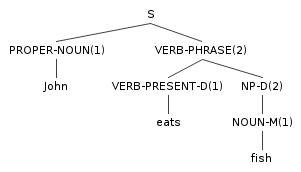
\includegraphics[scale=0.8]{john-eats-fish.png}
\end{figure}

... and reconstructing the derivation using the right-hand side of the rules this time, we obtain:

\begin{figure}[H]
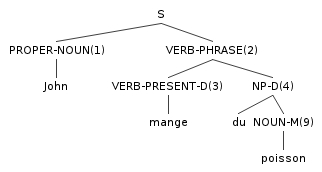
\includegraphics[scale=0.8]{john-mange-du-poisson.png}
\end{figure}

... which is also the only valid parse of `John mange du poisson', so the reverse translation must be correct.

Next we translate \begin{verbatim} Pierre does not eat fish \end{verbatim}

\begin{figure}[H]
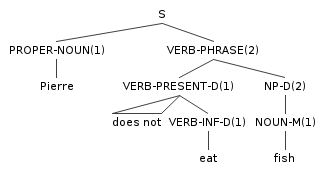
\includegraphics[scale=0.8]{pierre-does-not-eat-fish.png}
\end{figure}

... using the same procedure, we get:

\begin{figure}[H]
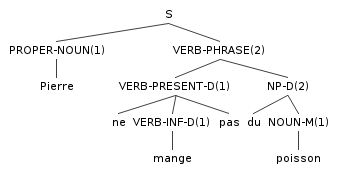
\includegraphics[scale=0.8]{pierre-ne-mange-pas-du-poisson.png}
\end{figure}

... as desired. Again, since this is the only parse for `Pierre ne mange pas du poisson', the reverse translation is correct too.

\begin{verbatim} Maria likes green apples \end{verbatim}

\begin{figure}[H]
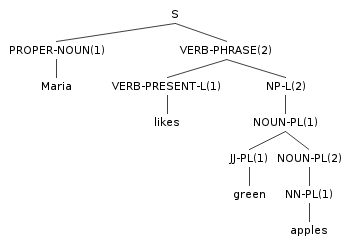
\includegraphics[scale=0.8]{maria-likes-green-apples.png}
\end{figure}
\begin{figure}[H]
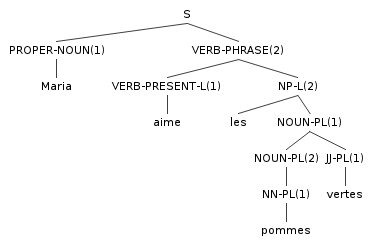
\includegraphics[scale=0.8]{maria-aime-les-pommes-vertes.png}
\end{figure}

\begin{verbatim} James thinks that Maria eats snails \end{verbatim}

\begin{figure}[H]
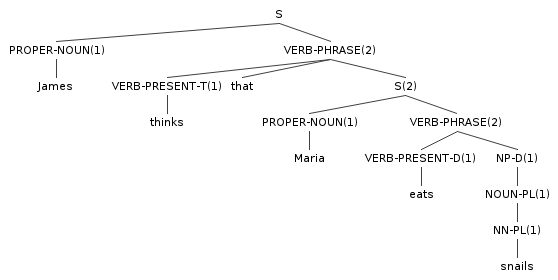
\includegraphics[scale=0.7]{james-thinks-that-maria-eats-snails.png}
\end{figure}
\begin{figure}[H]
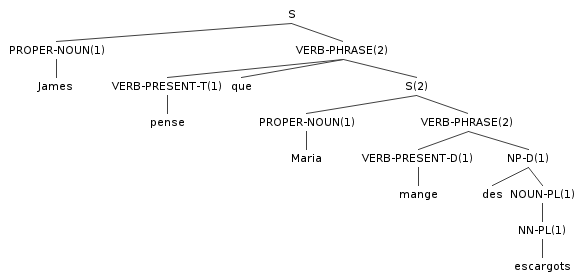
\includegraphics[scale=0.7]{james-pense-que-maria-mange-des-escargots.png}
\end{figure}

In each case the parse is unambiguous, so the translation works in both directions.

\begin{verbatim} John does not eat green apples \end{verbatim}
\begin{figure}[H]
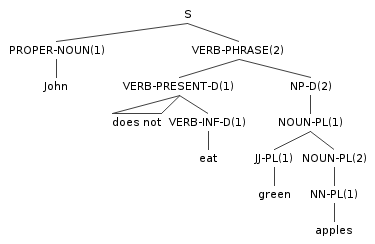
\includegraphics[scale=0.8]{john-does-not-eat-green-apples.png}
\end{figure}
\begin{figure}[H]
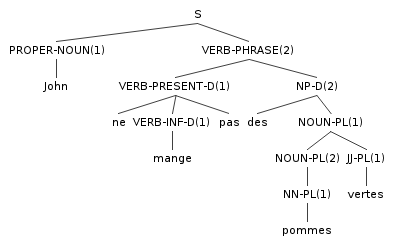
\includegraphics[scale=0.8]{john-ne-mange-pas-des-pommes-vertes.png}
\end{figure}

\begin{verbatim} James ne pense pas que Maria mange du poisson \end{verbatim}
\begin{figure}[H]
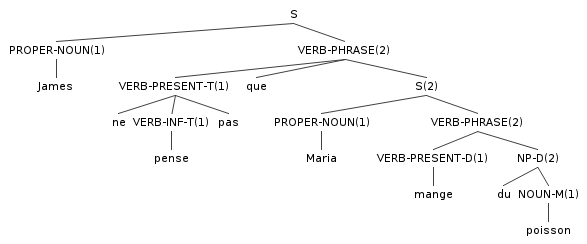
\includegraphics[scale=0.7]{james-ne-pense-pas-que-maria-mange-du-poisson.png}
\end{figure}
\begin{figure}[H]
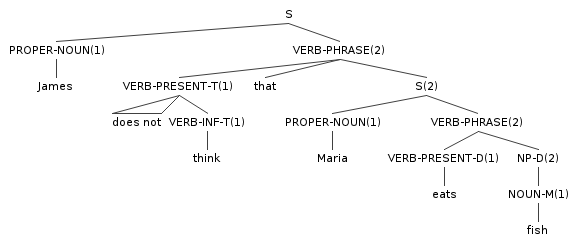
\includegraphics[scale=0.7]{james-does-not-think-that-maria-eats-fish.png}
\end{figure}

\section*{Question 3 (Sentiment Analysis and Opinion Mining)}
\subsection*{Overview}
The term `sentiment analysis' refers to the task of automatically determining,
given a text which expresses some opinion on some subject, to what degree that
opinion can be considered positive or negative. This concept can be applied on
the level of whole documents or to individual sentences, and naturally the two
problems are closely related. The following explanations focus more on the
problem at the document scope, since that is the problem that is most relevant
for assessing the favourability or otherwise of online product reviews.

Opinion mining is a related (and sometimes interchangeable) term which has
enjoyed a range of subtly different uses\cite{Pang2008}, but generally refers
to the broader problem of extracting, quantifying and analysing subjective
statements from a text.

There is much overlap between the problem domains of sentiment analysis and
opinion mining, and the methods outlined below are to some degree applicable in
both areas. However, we proceed with somewhat greater attention to sentiment
analysis, since that is the topic that is most directly relevant for high-level
monitoring of the reputation of a company.

\subsection*{Methods}

There is no single decisively superior method for performing sentiment
analysis. State-of-the-art approaches generally involve a combination of
techniques; this is to be expected since using a variety of techniques likely
means that less information is lost in the conversion from the raw data of a
document to whatever form is being analysed. The downside of this is that
achieving the best possible results requires a complex system which may take a
lot of work to implement. Rather than focusing on whole systems straight away,
we provide an overview of a number of the fundamental techniques available.

\subsubsection*{`Bag of words'}

Perhaps the most obvious approach that is applicable is what has become known
as the `bag of words' technique, in which the words contained within the
document are considered with no regard to their ordering; instead it is their
frequency which is used to determine a result. This idea can be used by
applying machine learning techniques directly to this frequency data (after
normalization), or as an assumption underlying more involved methods such as
`semantic orientation'.

The main advantage of bag-of-words is its simplicity - while it is a good
starting point for building more advanced techniques for sentiment analysis, by
itself it can be rather naïve. Since words are considered individually, the
phrase `not good at all' might be falsely taken to reflect positive sentiment,
for instance.

However, with appropriate learning methods, it is nevertheless possible to
achieve up to around 80\% accuracy with unigram models\cite{Pang2002}.
\subsubsection*{Semantic orientation}

In semantic orientation, significant words are each assigned a `polarity' or
`orientation' value which represents the degree to which they should be
considered positive or negative.

For instance, in a system where $1.0$ is maximally positive and $-1.0$ is
maximally negative, the word `good' might be assigned the value $0.9$ while
neutral words like `the' would be $0.0$. This table of polarity assignments
could potentially be constructed manually, but a better approach would be to
learn it from a set of example documents whose correct sentiment is already
known. Word-polarity learning is a somewhat separate problem, and is discussed
later.

Assuming the word polarities are already available, the remainder of the task
is to combine these values with the word frequencies from the document under
consideration, to produce an overall sentiment value.

One option is as follows: if $W$ is the set of words in the document, $f:W \to
\mathbb{N}$ maps words to their normalized frequencies, and $\Phi:W \to [-1,
1]$ their polarities, then an overall sentiment value is given by $\alpha =
\sum_{w \in W} f(w)\cdot\Phi(w)$.  \footnote{Note that this can be considered
as a scalar product in a real vector space; the situation is in fact analogous
to the linear NLP model used in question 1. This suggests the possibility of
learning word polarities using the averaged perceptron algorithm. However, there are
better options.}

\subsubsection*{Word presence}

An alternative to learning based on word frequencies is to use word
\emph{presence} as the base feature space. There are differing reports on
whether this conclusively produces better results\cite{Pang2002}, but it is
deserving of consideration.

\subsubsection*{Learning word polarities}

There are a wide variety of machine learning algorithms that have been adapted to the task of determining word sentiment. More detail is given in (Pang 2002)\cite{Pang2002}.

\textbf{Naive Bayes classifier}
A Bayes classifier relies on a strong independence assumption - i.e. that the
frequency of any one word does not depend on the frequency of any other word.
This is generally not an entirely valid assumption, but Bayes classifiers have
been shown to be surprisingly effective all the same.

\textbf{Maximum entropy classification}
Another probability-based classifier, but one which does not require independence assumptions and seeks to maximise the information entropy of the distribution at each stage. See (Pang 2002)\cite{Pang2002} for more detail. 

\textbf{The averaged perceptron algorithm}
(See question 1)
For our purposes, there is little reason to choose a perceptron over a Support
Vector Machine except that the perceptron method is generally easier to
implement, may be sufficient to produce reasonable results, and training may
be faster.

\textbf{Support Vector Machines}

SVM learning amounts to the process of finding a hyperplane which not only
separates the positive and negative examples in the feature space, but also
maximises the distance between the plane and the two classes.

\textbf{Assessment}

For sentiment analysis problems, SVMs generally appear to be a popular and
effective solution provided runtime is not the highest priority.

\subsubsection*{Bag of $n$-grams}
One obvious direction of improvement is to consider bigrams or $n$-grams in
place of individual words. This mitigates the problems caused by ignoring
context, but requires a larger training corpus to be effective since it makes
no attempt to infer general semantic rules; even with smoothing techniques,
unseen word combinations are likely to present difficulties.

\subsubsection*{Appraisal groups}
One technique which attempts to avoid some of the deficiencies resulting from
ignoring word ordering involves considering `appraisal
groups'\cite{Whitelaw2005} rather than individual words. This means that the
system attempts to group adjectives with their preceding modifiers - for
example, `tremendously boring' would be treated as one unit. The orientation
score for a group is then computed via a pre-constructed appraisal taxonomy (a
set of rules which assign base scores for adjectives and describe the effects
of various modifiers) applied to the group's component words.

Also of note is the fact that the appraisal groups method as described in the
paper attempts to classify the groups in more detail than just positive or
negative orientation. In addition, words may have `attitude', `graduation' and
other aspects which reflect more subtle properties of the sentiment expressed.
This provides a rich basis for features to be used for machine learning.

According to the experiments reported by the paper, using appraisal groups
combined with bag-of-words techniques can raise accuracy to around 90\% on some
datasets\footnote{ A Support Vector Machine with the Sequential Minimal
Optimisation algorithm was used for learning}, which is amongst the best
available.

A possible disadvantage of appraisal groups is the potential work involved in
constructing an effective appraisal taxonomy. While much of the process can be
automated, it is likely that some domain-specific fine-tuning would be required
in order for the method to produce good results.

\subsubsection*{Contextual polarity}
A related method, described in (Wilson 2005)\cite{Wilson2005} tracks a wide
array of textual features (for example, the number of adjectives in a sentence)
with the aim of using them to learn to determine how a word's context affects
its polarity\footnote{This is somewhat akin to learning of the appraisal
taxonomy in the above}. In fact, there are two sets of features, since the
procedure described uses two separate classification phases. The first
classification aims to separate neutral from polar terms, and the second is
applied to the polar terms to determine whether they are positive or negative.

Unfortunately, `contextual polarity' results are only available for
phrase-level sentiment analysis - while it seems promising, it is difficult to
compare directly to our other techniques. Applying some of the ideas from this
paper to a hybrid document-level approach has the potential to be very
effective, however.

\subsubsection*{Parser-based methods}
While some of the above methods attempt to deduce semantic relationships in the
text, they all stop short of applying parsing techniques. Since document
sentiment can be highly dependent on these semantic relationships, using a
parser to elucidate them is a logical step, and indeed perhaps an essential
component of any hypothetical perfect system.

(Nasukawa et al, 2003)\cite{Nasukawa 2003} uses a shallow parser combined with
a simple `sentiment dictionary' and some rules for modifiers (such as `not').
The results are mixed, but the system achieves 95\% precision on some datasets,
which indicates the potential rewards of deeper semantic analysis.

\subsubsection*{Assessing performance}

Any methodology for judging the performance of a system for sentiment analysis
will necessarily involve comparing the output classifications against some
known `gold-standard' classifications. Typical sources for such example data
include movie reviews in which a star rating is provided - in this case the
rating can reasonably be expected to reflect the correct sentiment assignment
for a review.

The preferred method for performing the comparison is \emph{ $n$-fold
cross-validation }. The available data is split into $n$ parts, and each part
is selected in turn for use as the test data, with the non-selected parts being
used for training. The overall performance measure is obtained by taking an
average of the accuracy percentages from the $n$ iterations.

\subsection*{b)}

\subsubsection*{System design}

As we have seen, there are many different approaches to the problem of
sentiment analysis, and the complexities of combining the various techniques
into a full system can make it difficult to determine what is useful and what
isn't.

The main two factors affecting the precision of a system are: a) the amount of
semantic information that is preserved in the process of reducing a document
from its raw text to the format used for analysis and b) the scope and quality
of the rules or features used to determine the sentiment value from this
format.  Provided both elements are sufficiently favourable, precision in
excess of 90\% should be achievable.

With this in mind, we consider a system which combines a detailed sentiment
lexicon as used for appraisal groups\cite{Whitelaw2005} with the semantic
information produced by a probabilistic natural language parser. This allows
the sentiment rules to depend on arbitrary features of the parse tree - for
instance, a rule might specify that the word `not' inverts the sentiment of its
sibling adjectival phrase.

Applying the various sentiment rules to the candidate parse trees will produce
a set of trees which are `tagged' with sentiment values. We then apply machine
learning to this data. The features used for learning can include the position
in the document as well as key words, so that the system can learn to give
extra weight to opinions given at the end of a review, or near the word
`overall', for example - should this prove to be helpful for classifying
documents.

As with appraisal groups, there is some difficulty in constructing a good
sentiment lexicon. One approach might be to use crowd-sourcing to tag parts of
documents according to perceived sentiment, and then compare the results with
the document's parse tree. It should be possible to extract rules from this
data using machine learning techniques (again). For example, a rule that `good'
reflects positive sentiment when used as an adjective but not as a noun could
be inferred from assigned sentiment values which reflect this usage.

This should be a very flexible system and, since it only builds on top of the
ideas of appraisal groups, should be no less effective. The extra information
conferred by a parser might even allow for improvements in accuracy, provided
similar care is taken over lexicon construction, so this direction seems like
one which is generally worthy of exploration.

\subsubsection*{Testing and usage}
In addition to the usual assessment practices (see above), a sensible policy
when using automated sentiment analysis as part of a real-world reputation
monitoring system would be to compare the results against data from more
traditional sources. For instance, polling customers directly for their
opinions on a product might give insight into the effectiveness of sentiment
analysis as applied to reviews of the same product over the same period. In
most cases one would hope that a successful sentiment analysis system would
reflect the same general opinion as that conveyed by the poll results, so any
significant disparity could be a sign that the system is not functioning
correctly, or is biased to some degree\footnote{Although for certain products,
it is less unusual for there to be such a difference: consider the case of a
film which is loved by the critics yet poorly received by the wider public}.

Another final consideration for real-world usage of the system is that in order
to accurately measure changes or trends in general sentiment over time, it is
important to bear in mind that any alteration in the data used for training has
the potential to skew the results. It is only reasonable to compare sentiment
values for different reviews which were produced by running the system with the
same training data. For this reason, the text of old reviews should be stored
so that their sentiment can be recomputed if improvements are made to the
training procedure or data.

\bibliography{Refs}{}
\bibliographystyle{plain}
\end{document}
